\documentclass[tikz]{standalone}

%实际大小 4096 x 2160
%centre (256,135)
%比例 16
%中心 2048,1080

\begin{document}

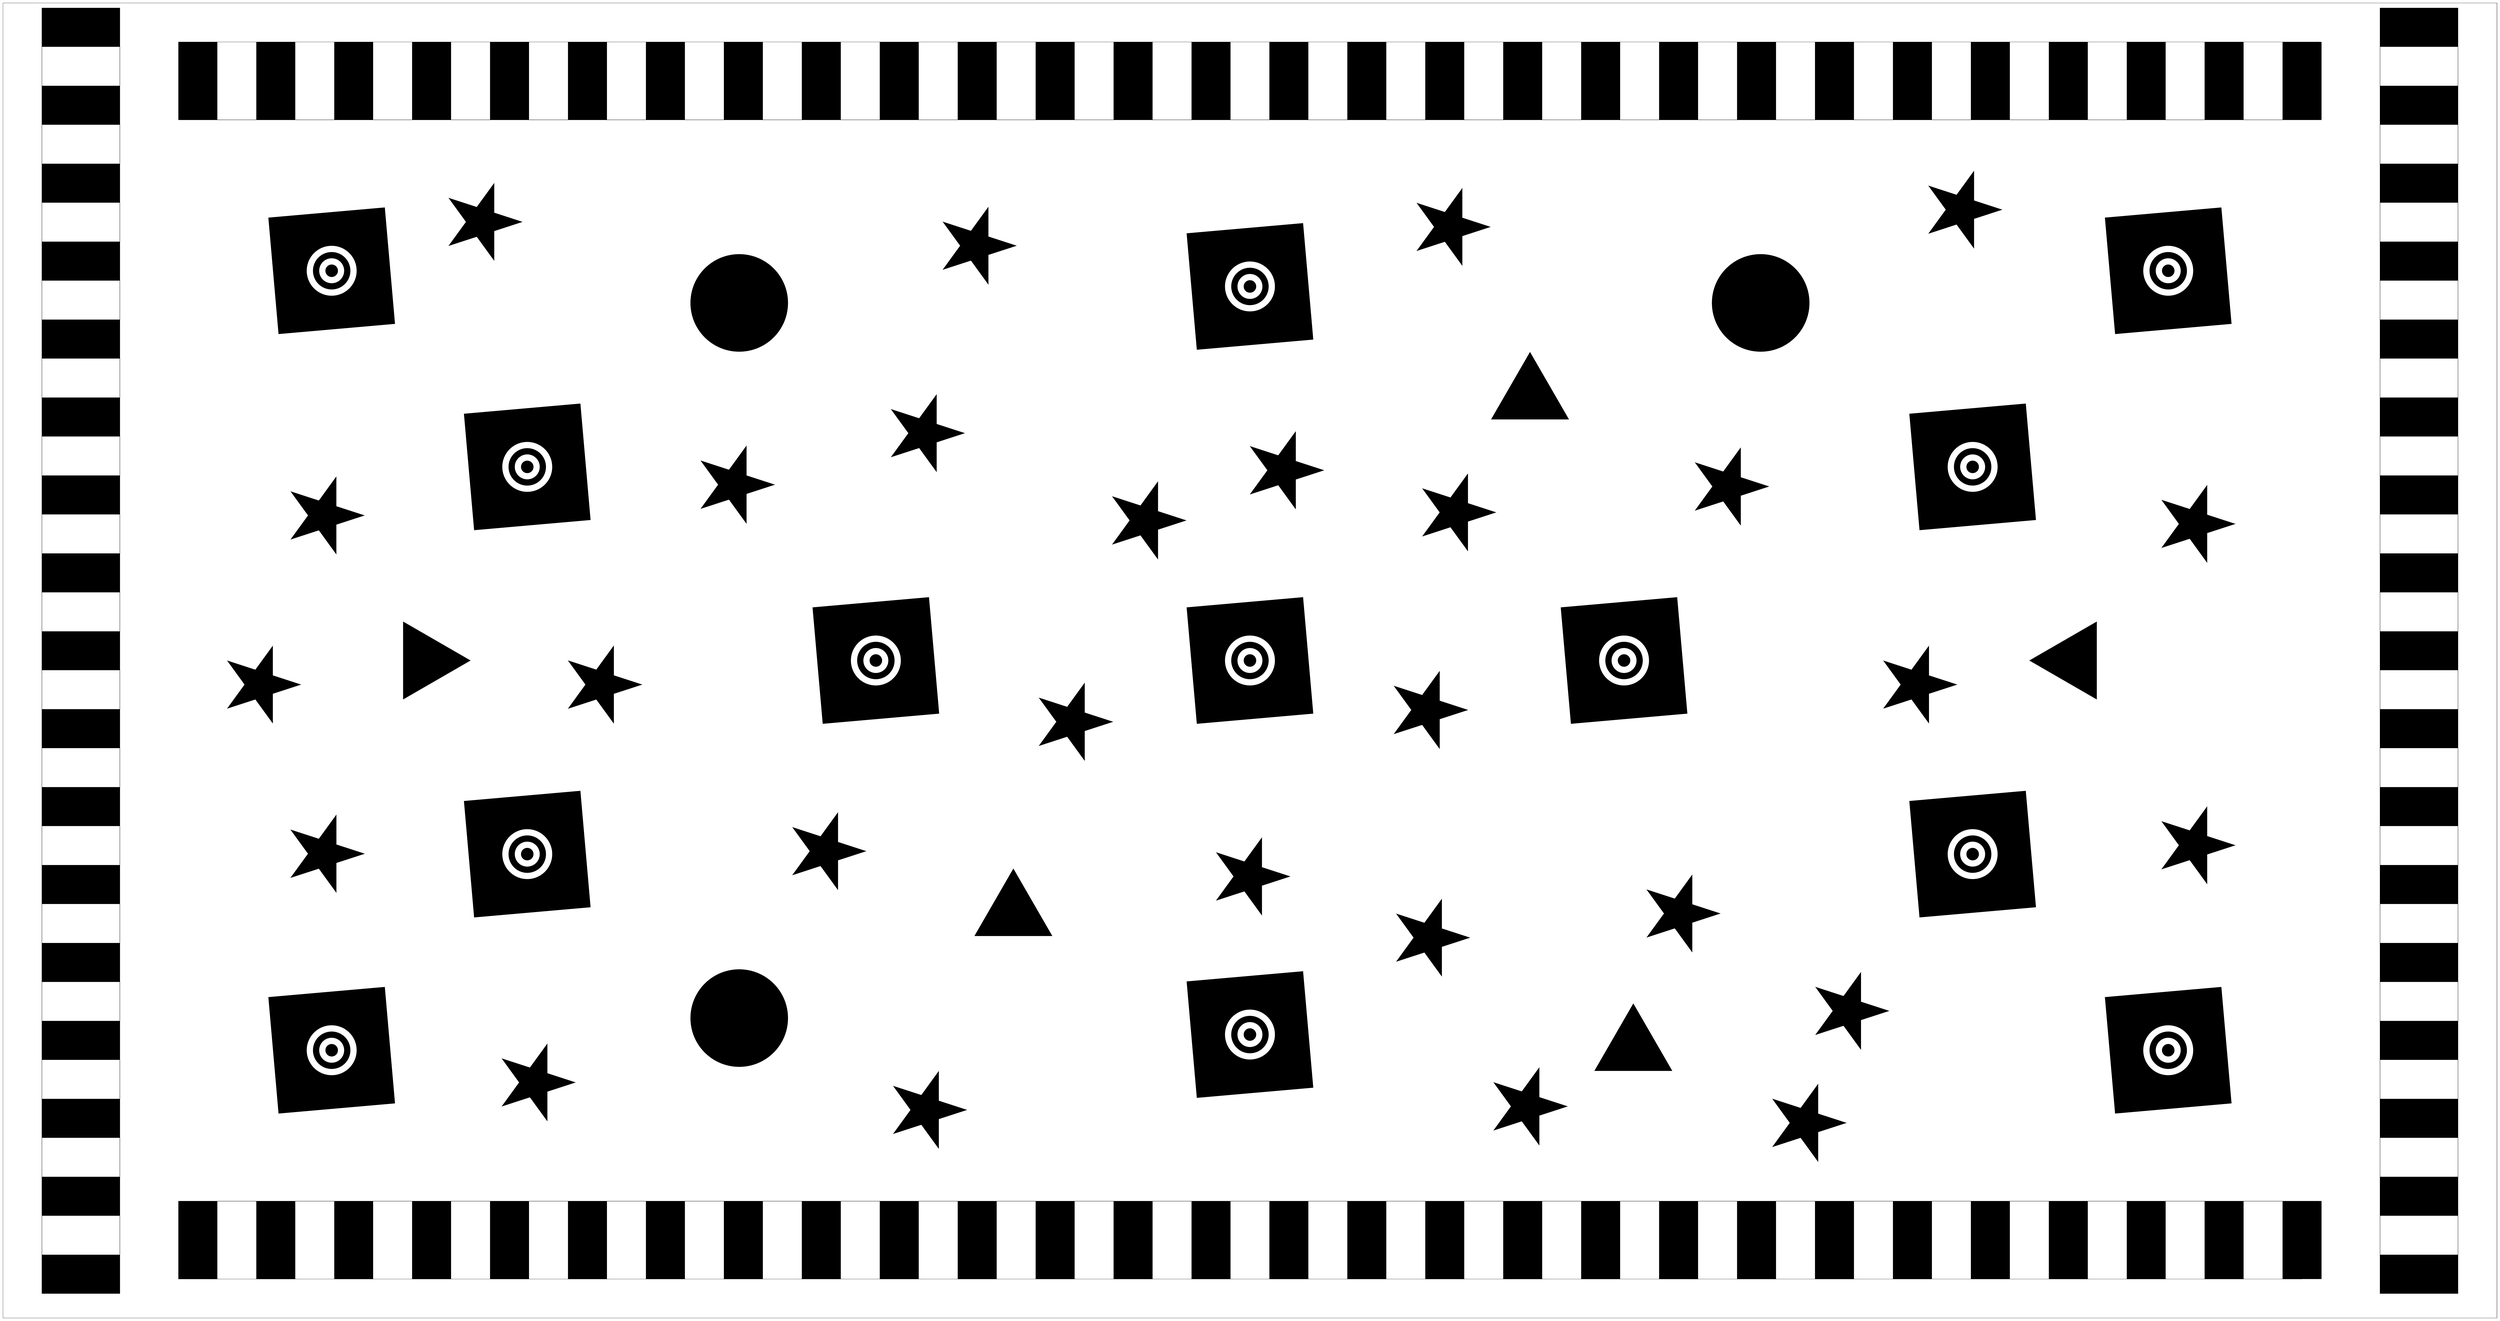
\begin{tikzpicture}[scale = 1.2]

\def\h{67.5}
\def\delta{10}
\def\r{128}
\def\square{6}
     


\newcommand{\wid}{4};    %small rectangle


\newcommand\rectanglepath{-- ++(\square,0) -- ++(0,\square) -- ++(-2*\square,0) -- ++(0,-2*\square)
-- ++ (2*\square,0) -- ++ (0,\square) -- cycle}  %big rectangle




\draw[use as bounding box,line width = 1,draw = black] (-1*\r,-67.5) rectangle (\r,67.5);   %画布大小
%\useasboundingbox[line width=2, black] (-1*\r-\delta,-67.5-\delta) rectangle (\r+\delta,67.5+\delta);

 %%%%%%%%%%%%%%%%%%%%% the three circle 
% \draw(0,0)circle(0.35*\r);%40
% \draw(0,0)circle(0.7*\r);%70
% \draw(0,0)circle(0.9*\r);    %100

%%%%%%%%%%%%%%%%%%cartesian coordinate
% \draw[->](90:100) -- (270:100);
% \draw[->](180:150) -- (0:150);




\draw[rotate around={5:(0,0)},fill=black,draw=none] (0,0) \rectanglepath;%center rectangle



%%%%%%%%%% 第一圈
\foreach \x in {0,90,180,270}
{
    \draw [rotate around={5:(\x:0.30*\r)},fill=black,draw=none] (\x:0.30*\r) \rectanglepath;
    
}

%\draw[fill=red,draw = none] (0,0) \circle(6);

%\draw [fill= red,draw = none](30:20)circle(0.35*\r);%40

%%第二圈
\foreach \x in {15,165,195,345}
{
    \draw [rotate around={5:(\x:0.6*\r)},fill=black,draw=none] (\x:0.6*\r) \rectanglepath;
}

%%第三圈
\foreach \x in {23,157,203,337}
{
    \draw [rotate around={5:(\x:0.8*\r)},fill=black,draw=none] (\x:0.8*\r) \rectanglepath;
}


%%%%%% 三个圆
\foreach \x in {35,145,215}
{
    \draw [fill = black] (\x:0.5*\r) circle (5);

}



%%%%%%%%%%%%%%%%%%%%%%%%%%%%%%%%%%%%%%%%%%%%%%%%%%%%%%%%%%同心圆
%第0圈


%\draw [fill= white,draw = none](0:0)circle(0.025*\r);%40
\draw [fill= white,draw = none](0:0)circle(0.02*\r);%40
\draw [fill= black,draw = none](0:0)circle(0.015*\r);%40
\draw [fill= white,draw = none](0:0)circle(0.01*\r);%40
\draw [fill= black,draw = none](0:0)circle(0.005*\r);%40


%第一圈
\foreach \x in {0,90,180,270}
{
    
    \draw [fill= white,draw = none] (\x:0.30*\r) circle(0.02*\r);%40
    \draw [fill= black,draw = none] (\x:0.30*\r) circle(0.015*\r);%40
    \draw [fill= white,draw = none](\x:0.30*\r)circle(0.01*\r);%40
    \draw [fill= black,draw = none](\x:0.30*\r)circle(0.005*\r);%40
    %\draw [fill= white,draw = none](\x:0.30*\r)circle(0.005*\r);%40

    
}


%第二圈
\foreach \x in {15,165,195,345}
{
    
    \draw [fill= white,draw = none] (\x:0.6*\r) circle(0.02*\r);%40
    \draw [fill= black,draw = none] (\x:0.6*\r) circle(0.015*\r);%40
    \draw [fill= white,draw = none] (\x:0.6*\r) circle(0.01*\r);%40
    \draw [fill= black,draw = none] (\x:0.6*\r) circle(0.005*\r);%40
    %\draw [fill= white,draw = none] (\x:0.6*\r) circle(0.005*\r);%40

    
}

%第三圈
\foreach \x in {23,157,203,337}
{
    \draw [fill= white,draw = none] (\x:0.8*\r) circle(0.02*\r);%40
    \draw [fill= black,draw = none] (\x:0.8*\r) circle(0.015*\r);%40
    \draw [fill= white,draw = none] (\x:0.8*\r) circle(0.01*\r);%40
    \draw [fill= black,draw = none] (\x:0.8*\r) circle(0.005*\r);%40
    %\draw [fill= white,draw = none] (\x:0.8*\r) circle(0.005*\r);%40

}




%%%%%%%%%%%%%%%%%%%%%%%%%%%%%%%%%%%%%%%%%%%%%%%%%%%%%同心圆



\renewcommand\rectanglepath{-- ++(0,\wid) -- ++(2*\wid,0) -- ++(0,-1*\wid)  -- cycle}  %重定义小方块



%%%%%%%%
%\newcommand\gap{4}
%%%%%%%%%%%%%%%%%%%%%%%%%%        left to right rectangle
\foreach \x in {-65,-57,...,66}
{
    \path[fill = black,draw = none](-1*\r+\wid,\x) \rectanglepath;
    % \path [fill = black,draw = none] (-1*\r+\wid,\x) \rectanglepath;
    % \path [fill = black,draw = none] (-1*\r+2*\wid,\x+\wid) \rectanglepath;


    \draw [fill=black,draw=none] (\r-3*\wid,\x) \rectanglepath;
    % \draw [fill=black,draw=none] (\r-2*\wid,\x) \rectanglepath;
    % \draw [fill=black,draw=none] (\r-\wid,\x+\wid) \rectanglepath;

}


\draw [line width = 1,black](-1*\r+\wid,-65) -- (-1*\r+\wid,67);
\draw [line width = 1,black] (-1*\r+3*\wid,-65) -- (-1*\r+3*\wid,67);
% \draw [line width = 1,black] (-1*\r,-65) -- (-1*\r+3*\wid,-65);

\draw [line width = 1,black](1*\r-\wid,-65) -- (1*\r-\wid,67);
\draw [line width = 1,black] (\r-3*\wid,-65) -- (\r-3*\wid,67);

% \draw [line width = 1,black](\r-3*\wid,-65) -- (\r-3*\wid,63);
% \draw [line width = 1,black] (\r,63) -- (\r-3*\wid,63);
% \draw [line width = 1,black] (\r,-65) -- (\r-3*\wid,-65);

\renewcommand\rectanglepath{-- ++(0,2*\wid) -- ++(\wid,0) -- ++(0,-2*\wid)  -- cycle}  %重定义小方块
% %%%%%%%%%%%%%%%%%%%%%%%%%%%  bottom to up rectangle

 \foreach \x in {-114,-106,...,106}
 {
     \draw [fill=black,draw=none] (\x+\wid,-1*\h+\wid) \rectanglepath;
%     \draw [fill=black,draw=none] (\x,-1*\h+\wid) \rectanglepath;
%     \draw [fill=black,draw=none] (\x+\wid,-1*\h+2*\wid) \rectanglepath;
    
     \draw [fill=black,draw=none] (\x+\wid,\h-3*\wid) \rectanglepath;
%     \draw [fill=black,draw=none] (\x+\wid,\h-2*\wid) \rectanglepath;
%     \draw [fill=black,draw=none] (\x,\h-\wid) \rectanglepath;
 }

 \draw [line width = 1,black](-110,-1*\h+3*\wid) -- (110,-1*\h+3*\wid);
\draw [line width = 1,black](-110,-1*\h+\wid) -- (108,-1*\h+\wid);
% \draw [line width = 1,black](102,-1*\h) -- (102,-1*\h+3*\wid);

\draw [line width = 1,black](-110,\h-3*\wid) -- (110,\h-3*\wid);
\draw [line width = 1,black](-110,\h-\wid) -- (110,\h-\wid);
% \draw [line width = 1,black](102,\h) -- (102,\h-3*\wid);




%%%%%%%配准
\newcommand\tri{-- ++(8,0) -- ++ (120:8) -- cycle}

\draw [fill=black,draw=none] (45:35) \tri;
\draw [fill=black,draw=none] (225:40) \tri;
\draw [fill=black,draw=none] (310:55) \tri;

\renewcommand\tri{-- ++(150:8) -- ++ (270:8) -- cycle}
\draw [fill=black,draw=none] (180:80) \tri;

\renewcommand\tri{-- ++(30:8) -- ++ (270:8) -- cycle}
\draw [fill=black,draw=none] (0:80) \tri;


%%%%%%%五角星
\newcommand\Radius{8}
\newcommand\pentagram{ -- ++ (90-144:\Radius)-- ++(90:\Radius)--++ (90+144:\Radius)-- ++
(90-72:\Radius)-- ++(90+72:\Radius)--cycle}

\draw [fill=black,draw=none] (0:65) \pentagram;
\draw [fill=black,draw=none] (45:25) \pentagram;
\draw [fill=black,draw=none] (35:85) \pentagram;


\draw [fill=black,draw=none] (10:95) \pentagram;
\draw [fill=black,draw=none] (70:50) \pentagram;
\draw [fill=black,draw=none] (125:55) \pentagram;
\draw [fill=black,draw=none] (145:45) \pentagram;
\draw [fill=black,draw=none] (170:100) \pentagram;
\draw [fill=black,draw=none] (150:95) \pentagram;
\draw [fill=black,draw=none] (170:100) \pentagram;

\draw [fill=black,draw=none] (180:105) \pentagram;
\draw [fill=black,draw=none] (200:50) \pentagram;

\draw [fill=black,draw=none] (208:87) \pentagram;
\draw [fill=black,draw=none] (230:57) \pentagram;

\draw [fill=black,draw=none] (300:30) \pentagram;
\draw [fill=black,draw=none] (330:47) \pentagram;

\draw [fill=black,draw=none] (330:67) \pentagram;


\draw [fill=black,draw=none] (350:95) \pentagram;


\draw [fill=black] (350:15) \pentagram;
\draw [fill=black] (90:22) \pentagram;
\draw [fill=black] (130:22) \pentagram;
\draw [fill=black] (190:22) \pentagram;
\draw [fill=black] (260:20) \pentagram;

\draw [fill=black] (24:50) \pentagram;
\draw [fill=black] (180:70) \pentagram;
\draw [fill=black] (160:60) \pentagram;
\draw [fill=black] (190:100) \pentagram;
\draw [fill=black] (320:70) \pentagram;
\draw [fill=black] (300:50) \pentagram;



\end{tikzpicture}

\newpage 

\end{document}